\section{Source Terms}

\begin{tabular*}{6.35cm}{|p{2.5cm}|p{3cm}|} \hline
Object acronym & ST \\
C++ class      & CSourceTerm \\
Source files   & rf\_st\_new.h/cpp \\
\hline
File extension & *.st \\
Object keyword &  {\#SOURCE\_TERM} \\
\hline
\end{tabular*}

\Developer{
%----------------------------------------------------------
\subsection{Theory}

In terms of the general balance equation for a quantity $\psi$,
source terms $\Source^\psi$ are defined in the following way
(Kolditz 2002, Chapter 1.2.3).
%
\begin{eqnarray}
\frac{d\psi}{dt}
=
\frac{\partial\psi}{\partial t}
+
\nabla \cdot {\bf\Phi}^\psi
=
\Source^\psi
\end{eqnarray}


\begin{table}[h]
%\caption{}
\begin{tabular}{|l|l|l|}
\hline
Subject & Symbol & Unit
\\
\hline
\hline
Fluid phase mass source term &
$\Source^{\Density^\Phase}$ &
$kg s^{-1}$
\\
Fluid phase volume source term &
$1/\Density^\Phase \Source^{\Density^\Phase}$ &
$m^3 s^{-1}$
\\
Heat source term &
$\Source^h$ &
$W s^{-1}$
\\
Mass source term (tracer, soluted, sorbed) &
$\Source^{\Conc_\Comp}$ &
$kg s^{-1}$
\\
Momentum source term (load, force) &
$\Source^m$ &
$N$
\\
Fluid mixture mass source term &
$\sum_\Phase \Source^{\Density^\Phase}$ &
$kg s^{-1}$
\\
Fluid mixture volume source term &
$\sum_\Phase 1/\Density^\Phase \Source^{\Density^\Phase}$ &
$m^3 s^{-1}$
\\
\hline
\end{tabular}
\end{table}
%
with:
$\Phase$ - fluid phase,
$\Comp$ - component.

}

%-------------------------------------------------------------------------------
\subsection{\texttt{\bf\#SOURCE\_TERM}}
\label{sec:st}
%\subsubsection{Keyword structure}

\begin{verbatim}
#SOURCE_TERM
 $PCS_TYPE // physical process
  LIQUID_FLOW       // H process (incompressible flow)
  GROUNDWATER_FLOW  // H process (incompressible flow)
  RIVER_FLOW        // H process (incompressible flow)
  RICHARDS_FLOW     // H process (incompressible flow)
  OVERLAND_FLOW     // H process (incompressible flow)
  GAS_FLOW          // H process (compressible flow)
  TWO_PHASE_FLOW    // H2 process (incompressible/compressible flow)
  COMPONENTAL_FLOW  // H2 process (incompressible/compressible flow)
  HEAT_TRANSPORT    // T process (single/multi-phase flow)
  DEFORMATION       // M process (single/multi-phase flow)
  MASS_TRANSPORT    // C process (single/multi-phase flow)
 $PRIMARY_VARIABLE
  PRESSURE1      // flow (phase)
  SATURATION2
  HEAD            // head
  TEMPERATURE1   // heat transport
  DISPLACEMENT_X1 // deformation  (radial direction for axisymmetry)
  DISPLACEMENT_Y1
  DISPLACEMENT_Z1  //(axial direction for axisymmetry)
  CONCENTRATION1 // mass transport
  CONCENTRATIONx
  EXCAVATION     // Simulation of excavation deformation
 $GEO_TYPE // geometry
  POINT    name
  POLYLINE name
  SURFACE  name
  VOLUME   name
 $DIS_TYPE // value distribution
  ANALYTICAL value1 value2 value3 // 4.2.13(CMCD)
  CONSTANT value
  CONSTANT_NEUMANN value
  LINEAR no_points
   Point1 value1
   Point2 value2
   Point3 value3
  LINEAR_NEUMANN no_points
   Point1 value1
   Point2 value2
   Point3 value3
  RIVER no_points
   Point1 HeadRiver KfRiverBed WidthRiverBed TopRiverBed BottomRiverBed
   Point2 HeadRiver KfRiverBed WidthRiverBed TopRiverBed BottomRiverBed
  CRITICALDEPTH
 $TIM_TYPE // time dependencies
  CURVE number
 $DIS_TYPE_CONDITION //4.3.20
  PCS pcs_type_name
\end{verbatim}


\begin{tabular*}{12.773cm}{|p{3.cm}|p{1.5cm}|p{7cm}|} \hline
Parameter          & Acronym & Meaning \\ \hline \hline
%
\texttt{PCS\_TYPE} & PCS &  Reference to a process \\
\texttt{GEO\_TYPE} & GEO &  Reference to a geometric object \\
\texttt{DIS\_TYPE} & DIS &  Distribution of source terms values \\
\texttt{TIM\_TYPE} & TIM &  Time dependencies of source terms \\
\hline
\end{tabular*}

\subsubsection{\texttt{\$PCS\_TYPE}}

\begin{tabular*}{12.773cm}{|p{3.cm}|p{1.5cm}|p{7cm}|} \hline
Parameter          & Value & Meaning \\ \hline \hline
%
\texttt{PRESSUREx}        & phase & Source term for fluid phase x \\
\texttt{HEAD}             & phase & Source term for fluid phase x \\
\texttt{DISPLACEMENTx\_X} & phase & Load force for solid phase x \\
\texttt{DISPLACEMENTx\_Y} & phase & ... \\
\texttt{DISPLACEMENTx\_Z} & phase & ... \\
\texttt{TEMPERATUREx}     & phase & Source term for temperature \\
\texttt{CONCENTRATIONx}   & component & Source term for component mass \\
\hline
\end{tabular*}

\subsubsection{\texttt{\$GEO\_TYPE}}

\begin{tabular*}{12.773cm}{|p{3.cm}|p{8.9cm}|} \hline
Parameter          & Meaning \\ \hline \hline
%
\texttt{POINT}     & Name of point \\
\texttt{POLYLINE}  & Name of polyline \\
\texttt{SURFACE}   & Name of surface \\
\texttt{VOLUME }   & Name of volume \\
\texttt{DOMAIN }   & whole domain \\
\hline
\end{tabular*}

\subsubsection{\texttt{\$DIS\_TYPE}}

\begin{tabular*}{12.773cm}{|p{3.cm}|p{8.9cm}|} \hline
Parameter          & Meaning \\ \hline \hline
%
\texttt{ANALYTICAL}        & matrix diffusion as analytical solution \\
\texttt{CONSTANT}          & value is assigned to each node found \\
\texttt{CONSTANT\_NEUMANN} & value times node area/node length is assigned to each node found \\
\texttt{LINEAR}            & linear distribution of values is assigned to each node found \\
\texttt{LINEAR\_NEUMANN}   & linear distribution of values times node length or area is assigned to each node found  \\
\texttt{RIVER}   & linear distribution of values times node length
or area is assigned to each node found,
                   terms depend on groundwater head and the river parameters \\
\texttt{CRITICALDEPTH}   & Dynamic source for Overland Flow, term depends on head\\
\texttt{SYSTEM\_DEPENDENT}  & free seepage face \\
\hline
\end{tabular*}

\subsubsection{\texttt{\$TIM\_TYPE}}

\begin{tabular*}{12.773cm}{|p{3.cm}|p{8.9cm}|} \hline
Parameter           & Meaning \\ \hline \hline
%
\texttt{CURVE}      & TIM curve number \\
\hline
\end{tabular*}

\subsubsection{\texttt{\$DIS\_TYPE\_CONDITION}}

\begin{tabular*}{12.773cm}{|p{3.cm}|p{8.9cm}|} \hline
Parameter           & Meaning \\ \hline \hline
%
\texttt{PCS pcs\_type\_name} & source term provided from coupled process \texttt{pcs\_type\_name}\\
\hline
\end{tabular*}



\Examples{
%-------------------------------------------------------------------------------
\subsection{Examples}

%%WW
\subsubsection{Excavation deformation}
\label{sec:st_excav}
If a process is defined as excavation deformation simulation in .pcs file (see Section \ref{sec:pcs_dm}).
 The domains to be excavated  can be defined in this file by polylines or surfaces. Here is an example of such
 input data:
\begin{verbatim}
#SOURCE_TERM
 $PCS_TYPE
  DEFORMATION
 $PRIMARY_VARIABLE
  EXCAVATION
 $GEO_TYPE
  POLYLINE PLY_9
  EXCAVATION_DOMAIN 2
\end{verbatim}
where keywords POLYLINE or SURFACE define cave surface for 2D and 3D problems, respectively. Meanwhile keyword
 "EXCAVATION\_DOMAIN" and the following integer specifies patch index such that all elements that have this
   patch index are assumed in the domain to be excavated. The reason to put these data in .st file is
     that such data defile surfaces of caves and released loads will be applied to these surfaces as Neumann,
      or traction boundary conditions for excavation simulation.

\subsubsection{Source at point}

\begin{verbatim}
benchmark: h_line.st
#SOURCE_TERM
 $PCS_TYPE
  LIQUID_FLOW
 $PRIMARY_VARIABLE
  PRESSURE1
 $GEO_TYPE
  POINT POINT0
 $DIS_TYPE
  CONSTANT 1.157407e-006
#STOP
\end{verbatim}

This source term is defined for a process with primary variable
PRESSURE1. Geometrically the source term is linked to point 0
named POINT0.

\begin{verbatim}
benchmark: h_line.gli
#POINTS
0 0.0 0.0 0.0
#STOP
\end{verbatim}

\subsubsection{Source along polyline}

\begin{verbatim}
benchmark: h_tet3.st
#SOURCE_TERM
 $PCS_TYPE
  LIQUID_FLOW
 $PRIMARY_VARIABLE
  PRESSURE1
 $GEO_TYPE
  POLYLINE BOREHOLE
 $DIS_TYPE
  CONSTANT 1.157407e-000
#STOP
\end{verbatim}

This source term is defined for a process with the primary
variable PRESSURE1. Geometrically the source term is linked to a
polyline named BOREHOLE.

\begin{verbatim}
benchmark: h_tet3.gli
#POINTS
0 0.0 0.0 -10.
1 0.0 0.0  10.
#POLYLINE
 $NAME
  BOREHOLE
 $TYPE
  0
 $EPSILON
  0.060000e+000
 $POINTS
  0
  1
#STOP
\end{verbatim}

The polyline BOREHOLE is defined by two points 0 and 1.

\subsubsection{Source along polyline}

This is an example for source terms (load force) along a polyline
for a deformation process. The value is equally distributed along
the polyline named TOP. Additionally the source has a time
dependency according to time curve 2 (see section \ref{sec:tim}).

\begin{verbatim}
benchmark: h_cc_tri.st
#SOURCE_TERM
 $PCS_TYPE
  DEFORMATION
 $PRIMARY_VARIABLE
  DISPLACEMENT_Y1
 $GEO_TYPE
  POLYLINE TOP
 $DIS_TYPE
  CONSTANT_NEUMANN -1.0
 $TIM_TYPE
  CURVE 2
#STOP
\end{verbatim}

\subsubsection{River}
This is an example for a River source terms along the polyline
Channel. The polyline may contain more than 2 point; data points
with river parameters only are defined for 2 points 4 and 5. A
linear interpolation of all parameters is done automatically.

\begin{verbatim}
benchmark: h_riv1_pris.st
#SOURCE_TERM
 $PCS_TYPE
  HEAD
 $GEO_TYPE
  POLYLINE Channel
 $DIS_TYPE
  RIVER 2
  4  3 1.00e-6 60.0 1.3 1.0
  5  3 1.00e-6 60.0 1.3 1.0
#STOP
\end{verbatim}

For the case of Head aquiver $ > $ Bottom RiverBed the equation
for the river source term is:

\begin{verbatim}
q = (RiverConductance * HRiver) - (RiverConductance * HAquifer)
\end{verbatim}

The first term is added as RHS term to the equation system, the second
term is added on the diagonal using the function MXInc(). For the
case of Head aquiver $ < $ Bottom RiverBed the equation for the
river source term is:

\begin{verbatim}
Haquiver  <  BRiverBed q = (RiverConductance * HRiver)   -
(RiverConductance * BRiverBed)
\end{verbatim}

Both terms are added to the RHS as 'normal' source terms. River conductance is defined as:

\begin{verbatim}
RiverConductance = KfRiverBed* WidthRiverBed* NodeReachLength /
                   TopRiverBed - BottomRiverBed
\end{verbatim}

\subsubsection{Data input from EXCEL files}

Fig. \ref{fig:st_excel} shows an EXCEL file for well data. This
data can be imported using the \texttt{\#DATA\_BASE} option. The
EXCEL file has to be converted to a CSV file before data
processing.

\begin{figure}[htb!]
  % Requires \usepackage{graphicx}
  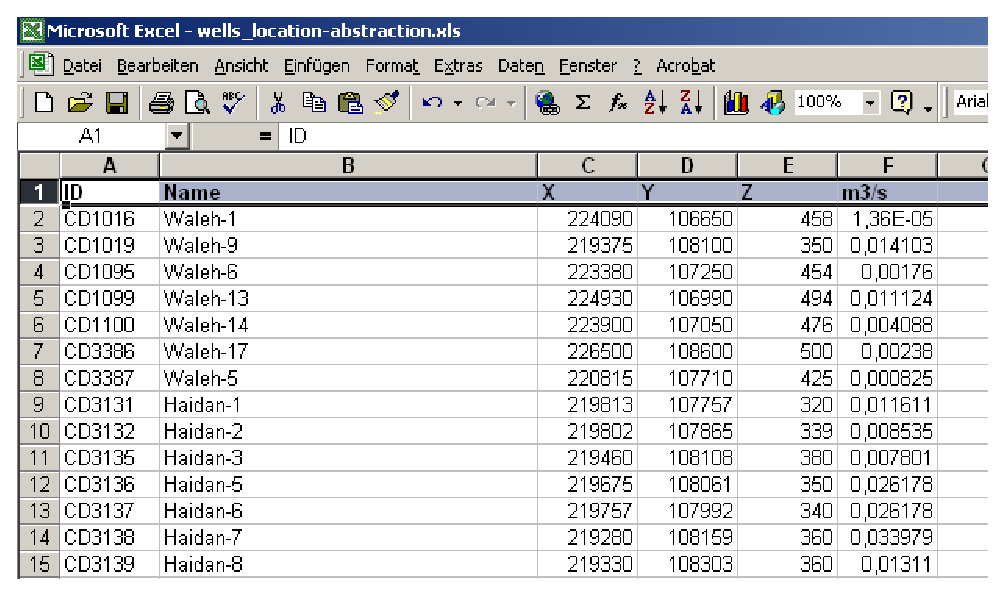
\includegraphics[width=12cm]{figures/st_data_base.eps}\\
  \caption{EXCEL sheet for well data import}
  \label{fig:st_excel}
\end{figure}

\subsubsection{Analytical source term}
This is an example for a fracture plane in a rock body. Here the
solution is applied to two processes, heat transport and mass
transport. The \$PCS\_TYPE defines the process for which the
source term is to be applied. The \$GEO\_TYPE specifies DOMAIN
indicating all nodes in the specified material group (value 1) act
as sources.

\begin{verbatim}
benchmark: frac_an.st
#SOURCE_TERM
 $PCS_TYPE
  MASS_TRANSPORT
 $PRIMARY_VARIABLE
  CONCENTRATION1
 $GEO_TYPE
  DOMAIN
 $DIS_TYPE
  ANALYTICAL 0 1.e-6 50

#SOURCE_TERM
 $PCS_TYPE
  HEAT_TRANSPORT
 $PRIMARY_VARIABLE
  TEMPERATURE1
 $GEO_TYPE
  DOMAIN
 $DIS_TYPE
  ANALYTICAL 0 1.e-3 50
\end{verbatim}

Three variables are required

value 1: material group of the fracture

value 2: diffusion constant in matrix

value 3: number of previous time steps to be taken into account
(max 50).

The method will be documented in a forthcoming publication. It is
currently only available for triangular and quadratic elements
acting as 2D elements in 3D space, here representing fractures in
matrix.

\LastModified{CMCD - 19th December 2005}
